\documentclass[a4paper, 12pt]{article}
\usepackage[top=1.2in, bottom=1.2in, left=1.0in, right=1.0in]{geometry}
\usepackage[utf8]{inputenc}
\usepackage[english]{babel}
\usepackage[document]{ragged2e}
\usepackage{multicol}
\usepackage{multirow}

\usepackage[bookmarksopen=true, hidelinks]{hyperref}
\usepackage{bookmark}
\bookmarksetup{numbered}

\usepackage{cite}
\usepackage{acro}

\newcommand{\acdef}[2]{
	\DeclareAcronym{#1}{
		short = #1,
		long = #2,
	}
}
\acdef{3AC}{Three-Address Code}
\acdef{AFG}{Aggregate Flow Graph}
\acdef{CFG}{Contract Flow Graph}
\acdef{CLI}{Command Line Interface}
\acdef{DTA}{Dynamic Taint Analysis}
\acdef{EPC}{Enclave Page Cache}
\acdef{JLS}{Java Language Specification}
\acdef{JNI}{Java Native Interface}
\acdef{JVM}{Java Virtual Machine}
\acdef{LFG}{Local Flow Graph}
\acdef{OOP}{Object-oriented Programming}
\acdef{SGX}{Software Guard Extension}
\acdef{TEE}{Trusted Execution Environment}


\usepackage{wrapfig}
\usepackage{listings}
\lstdefinestyle{j}{
	keywordstyle=\textbf,
	basicstyle=\ttfamily\scriptsize,
	tabsize=4,
	numbers=left,
}

\usepackage{amsmath}
\usepackage{amsthm}
\theoremstyle{definition}
\newtheorem{defin}{Definition}

\usepackage{xcolor}
\usepackage{soul}

\usepackage{sourcecodepro}

\usepackage{csquotes}

\usepackage[pdf]{graphviz}

\title{Data flow analysis for Uranus applications}
\author{Chan Kwan Yin (3035466978)}
\date{\today}


\newcommand{\IncludeCode}[5]{
  % \begin{wrapfigure}{r}{#4\textwidth}
  % \begin{minipage}{#4\textwidth}
  % \vspace{-#5 em}
  \begin{center}
    \lstinputlisting[style=j, language=java, label={#1}, caption={#3}]{#2}
  \end{center}
  % \vspace{-#5 em}
  % \end{minipage}
  % \end{wrapfigure}
}

\newcommand{\IncludeCodePart}[5]{
  \begin{center}
    \lstinputlisting[
    style=j,
    language=java,
    label={#1},
    caption={#3},
    firstline={#4},
    lastline={#5},
    ]{#2}
  \end{center}
}

\newcommand{\q}[1]{\enquote{#1}}

\newcommand{\pname}{\textit{enclavlow}}

\newcommand{\fnname}[1]{\underline{#1}}

\definecolor{code}{rgb}{0.95, 0.95, 0.95}
\sethlcolor{code}
\newcommand{\code}[1]{\colorbox{code}{\texttt{\footnotesize #1}}}

\begin{document}
% title page
\begin{titlepage}
	\begin{center}
		\vspace*{1em}
		\Huge
		\textbf{Data flow analysis for Uranus applications}

		\Large
		\vspace{1.5em}
		\textbf{Chan Kwan Yin (3035466978)}

		\vspace{0.5em}
		28 October 2020
	\end{center}
\end{titlepage}


% abstract page
\thispagestyle{empty}
\begin{abstract}
	Trusted Execution Environments (TEE) protect applications from privileged attacks
	running on untrusted systems such as public clouds,
	but partitioning enclave boundaries is not always a trivial task.
	Partitions too small would leak data to the untrusted host system,
	while partitions too huge would result in unnecessarily large trusted computing base (TCB)
	that increases the risk of overflowing Enclave Page Cache (EPC).
	A passive analysis approach can be adopted where
	users annotate data as sensitive sources or sinks,
	and an analysis tool determines variables considered sensitive
	and compares it with the enclave boundaries declared.

	This project introduces \pname{}, an information flow analysis tool
	for JVM-based projects using Intel SGX enclaves with the Uranus
	\footnote{ Uranus: Simple, Efficient SGX Programming and its Applications.
	\url{https://doi.org/10.1145/3320269.3384763}
	} framework.
	It implements a set of security policies tailored for Uranus-based applications,
	and reports leaking variables or functions that could be run out of enclave.
	The analysis tool is delivered as a Gradle plugin
	to be deployed as a continuous integration tool in Gradle-based projects.
	The source code for \pname{} is released on \url{https://github.com/SOF3/enclavlow}.
\end{abstract}

\newpage

% table of contents
\thispagestyle{empty}
\setlength\columnsep{3em}
\begin{multicols}2
  \footnotesize

	\tableofcontents
	\listoffigures
	\listoftables
	\lstlistoflistings

	\printacronyms[
		name = Abbreviations
	]
\end{multicols}

% main body
\setcounter{page}0
\newpage
\setlength\parskip{1.3em}

\section{Introduction}\label{sec:introduction}
\subsection{Background}\label{subsec:background}
With the rise of third-party public cloud services
such as \ac{AWS}~\cite{aws} and Microsoft Azure~\cite{azure},
there is increasing demand for trusted execution where
applications are protected from
attackers with privileged access to the hardware or software.
Modern hardware offer \ac{TEE} technologies,
such as \ac{SGX} in Intel CPUs,
with which trusted execution code and sensitive data
are processed in secure \q{enclaves},
protected at hardware level to prevent access
from other hardware or software layers.

One significant application of \ac{TEE} is the big data industry,
in which confidential user data are processed on cloud servers,
and protection from cloud providers may be necessary
for compliance with privacy regulations such as GDPR~\cite{gdpr}.
However, a significant amount of big data libraries and frameworks are written
using languages that use \ac{JVM} as the runtime,
such as Hadoop~\cite{apachehadoop} and Spark~\cite{apachespark}.
Recently, Uranus~\cite{uranus}, a system for
writing \ac{SGX} applications in Java languages, was released.
It provides a simple interface for interacting with \ac{SGX} in Java,
where users annotate methods with \code{@JECall} and \code{@JOCall}
to move control flow into or out of enclaves.
It is the responsibility of the user to determine the correct positions
for the \code{@JECall} and \code{@JOCall} annotations,
namely the enclave boundary partitioning.
Since \ac{JVM} involves a very different approach compared to native applications
in terms of software development, distribution and execution,
tools designed for native applications are mostly incompatible in \ac{JVM}.

One important question in enclave programming is the choice of an appropriate enclave boundary.
Running the whole application within an \ac{SGX} enclave is undesirable for two reasons.
First, this violates the Principle of Least Privilege,
where the whole application becomes possible attack surface
for adversaries to compromise protected data~\cite{glamdring}.
Second, this implies all memory used by the application
is placed in the enclave memory (the \ac{EPC}),
which is restricted to 100 MB,
the overflow of which results in swap memory mechanism,
leading to significant performance degrade
(\q{1,000X slowdown compared to regular OS paging}~\cite{uranus}).
On the other hand, if the enclave is smaller than necessary,
adversaries can either obtain sensitive data directly or
infer sensitive characteristics of them indirectly.
An enclave boundary is to be selected with high precision to avoid impacts from either side.
Ideally, the enclave boundary shall cover the minimum subset of code
in which sensitive data are processed
such that use of \ac{EPC} is minimized
without resulting in any sensitive data leak.

This project presents \pname{}
\footnote{\q{enclavlow} is a term coined from the words \q{enclave} and \q{flow}.},
an information flow analysis tool
for identifying data leak from enclaves.
The user first wraps sensitive data sources in \code{sourceMarker} and sinks in \code{sinkMarker}.
The tool performs information flow analysis from \code{sourceMarker} variables,
identifying the ways that data from such variables are leaked
to the system outside the executing enclave
without first passing through a \code{sinkMarker} variable.
The tool compiles a report in HTML format
that lists the flow of sensitive data leak
from the source marker to areas accessible by privileged adversaries.

\pname{} is shipped as a Gradle plugin,
providing a Gradle task that
takes the \code{*.class} files compiled in the \code{classes} task
and generates the report for the analysis from those classes.

\subsection{Prior work}\label{subsec:prior-art}
Information flow analysis is not a new technology in the field.
While this project analyzes \ac{JVM} code using \ac{SGX} enclaves,
prior research on \emph{automatic partition} and non-SGX dynamic analysis was found.

Glamdring~\cite{glamdring} is a C framework that
automatically selects the minimal \ac{SGX} enclave boundaries
based on user requirements specified through C pragma directives.
However, since the process is fully automated,
it has a lower tolerance of false positives,
which increases the risk of unintentional data leak.
This project, unlike Glamdring, will only perform analysis but not automatic partitioning,
allowing for greater false positive tolerance.

Phosphor~\cite{BellJonathan2014Pidd} is a \ac{DTA} framework
that modifies Java bytecode to add tags to sensitive data at runtime
and check if such tags are leaked.
Although dynamic taint is more accurate,
this project prefers a static analysis approach,
which enables developers to identify sensitive regions at compile time
without the need to feed concrete data into methods.

Civet~\cite{civet} is a framework for Java code partitioning.
Similar to Glamdring, it automatically selects the minimal enclave boundaries.
It is also similar to the goal of this project,
except that Uranus provides additional protection at the native level,
allowing further optimizations compared to Civet.
Challenges found in this project, such as polymorphism complexity, were also observed with Civet.

This report will focus on the algorithm used to detect data leaks,
as well as performance concerns and limitations from the \ac{JVM} design.
An example application is evaluated to demonstrate the functionality of \pname{}.


\section{Objectives}\label{sec:objectives}
This section describes the usage and intended behaviour of \pname{}.

\subsection{Marker API}\label{subsec:marker-api}
The \code{enclavlow-api} Gradle submodule in the project
is a library exposing two identity functions as expression markers
as shown in Listing~\ref{lst:source-sink-def}.
Corresponding definitions such as \code{intSourceMarker}
are also defined for the eight Java primitive types
for both source and sink (omitted in Listing~\ref{lst:source-sink-def} for brevity).
Users can wrap \emph{ultimate} sensitive data sources with \code{sourceMarker}
and mark \emph{intended} leaks with \code{sinkMarker}.
It is expected that the identity wrapper function is optimized away by \ac{JIT}.

\IncludeCode{lst:source-sink-def}{./SourceSinkDef.java}
{Definition of \code{sourceMarker} and \code{sinkMarker}}{.55}{3}

Exceptions induced from the expression of parameters to \code{sinkMarker}
are not collected by the sink.
This is because throwing sensitive data is a rare use case,
has a wide range of scenarios
and highly depends on the exact class thrown.
If sensitive information in an exception is intended for leaking,
a more verbose catch-wrap-throw syntax can be used
as demonstrated in Listing~\ref{lst:catch-wrap-throw}.
\code{sinkMarker} can also be used to explicitly suppress false positives generated by \pname{}.

\IncludeCode{lst:catch-wrap-throw}{./catch-wrap-throw.java}
{Catch-wrap-throw construct}{.35}{1}

A simple example usage is shown in Listing~\ref{lst:SourceSinkExample}.
In particular:
\begin{itemize}
  \item On line 4, \code{raw} is not \code{sourceMarker}
    because parsing is a late stage after raw data extraction
    and \code{sourceMarker} should only be applied on the ultimate source,
    which is asserted on line 5 that \q{computing the sum of \code{raw} is a legitimate leak}.
  \item \code{result} on line 14 is not marked \code{sinkMarker}
    because the leak of sensitive information should be analyzed.
    \code{sum} on line 22 is not marked \code{sinkMarker}
    because it is a sensitivity-neutral utility function
    that does not imply any assertion on whether the leak is acceptable;
    otherwise incorrect behaviour is created by changing line 12 to Listing~\ref{lst:computeSum},
    where \code{parse} no longer returns a security-sensitive value.
\end{itemize}

\IncludeCode{lst:SourceSinkExample}{./SourceSinkExample.java}
{Simple example of \code{sourceMarker} and \code{sinkMarker}}{.6}{2}

\IncludeCode{lst:computeSum}{./computeSum-example-leak.java}
{Example of leak through \code{computeSum}}{.55}{2.5}

\subsection{User interface}\label{subsec:user-interface}
The \code{enclavlow-plugin} Gradle submodule
is a Gradle plugin providing a task \code{:enclavlow},
which depends on the \code{:classes} builtin task
and performs flow analysis on the class binaries.
The analysis report is generated as HTML format in the Gradle reports directory
(build/reports/enclavlow.html).
The report contains the following elements:

\paragraph{Flow summary}
Each method that sensitive data flow through are reported.
If multiple invocations lead to different data flows,
the union of such data flows is displayed.

\paragraph{Data leaks}
Code that which results in immediate data leaks,
such as methods passing security-sensitive data to other \code{@JOCall} methods
or methods marked \code{@JECall} returning/throwing security-sensitive data,
are highlighted in an index called \q{Sensitive leaks}.
For each highlighted method, the developer
should move it into enclave boundaries,
or adjust the \code{sourceMarker}/\code{sinkMarker} wrappers.

\paragraph{Contract graphs}
The contract graph of each method is provided as hyperlinks in the HTML report
and can be viewed using the Graphviz Online tool \cite{dreampuf}.

When debug mode is enabled, the \ac{LFG} (see section \ref{subsubsec:lfg})
of each method can also be viewed in DOT/SVG format from \code{lfgOutput}
under the Gradle build directory.

\subsection{Threat model}\label{subsec:threat-model}
The adversary of concern is expected privileged access to the host system,
including other threads in the \ac{JVM} runtime, the \ac{JVM} runtime itself,
other (root) processes, the operating system kernel,
the hypervisor and the BIOS.
The adversary cannot access the \ac{SGX} execution part of the CPU
as cryptographically provable by SGX attestation mechanism.
While the realistic adversary also has access to hardware resources
such as system clock and temperature sensor modules,
which can be used to implement side-channel attacks,
analyzing such side channels involves
system-, environment-~and architecture-dependent analysis.
As these side channels rarely expose meaningful and specific information,
they are beyond the scope of this project.

The security model provided by Uranus is also slightly altered.
Uranus rejects assignment to objects outside enclaves
to mitigate some attacks like the Iago attack.
On the other hand, \pname{} considers such writes to be rvalue-leaking and control-flow-leaking,
but still assumes them permissible.
This change intends to target future changes in Uranus
that perform compile-time flow analysis.


\section{Methodology}
The main component of this project is the analysis framework,
which is conducted in the form of iterations
to fulfill security policies as specified in the integration tests.
Other parts such as Gradle plugin interfae,
although necessary for usage,
are not focus areas of this project, and hence will not be discussed further.

\subsection{Design}\label{subsec:design}
Since the adversary has arbitrary access to any untrusted memory and instruction,
the security policies of \pname{} differ slightly from typical information flow analysis.
For instance, the statement \code{a.b.c = d;} usually
does not propagte the effect of \code{d} to \code{a},
but since the adversary is capable of changing \code{b} to any memory location of its favour,
the security of this statement depends on whether \code{a} is trusted.

\pname{} adopts a flow graph approach,
where each node represents an element that may be leaked.

\begin{defin}
	Given a flow graph $(V, E)$, for all $x, y \in V$,
	$(x, y) \in E$ in a flow graph if and only if
	allocating $y$ outside an enclave reduces the indistinguishability of $x$.
\end{defin}

Note that this definition (\q{our definition}) differs slightly from
the usual definition of flow graphs (especially in DTA),
where an edge $(x, y)$ represents the flow of information from $x$ to $y$ ~\cite{YinHeng2007Pcsi}.
In the usual definition, only adversary read access to $y$ is concerned,
while in our definition, the adversary possesses write access to $x$.

\subsubsection{Contract flow graph (CFG)}
\pname{} adopts an approach where a CFG is constructed for each method analyzed.
The CFG contains the following nodes:
\begin{itemize}
	\item \q{Static}: Represents data located in static class fields
	\item \q{This}: Represents the object on which a method was invoked
	\item \q{Param $x$}: Each parameter is represented by a node
	\item \q{Return}: Represents data flow through the return path
	\item \q{Throw}: Represents data flow through the return path
	\item \q{Source}: Represents variables in the method explicitly wrapped in \code{sourceMarker}
	\item \q{Sink}: Represents locals in the method explicitly declared as \code{sinkMarker}
	\item \q{Control}: This is a special node representing how many times the function is called.
	\item \q{This}, \q{Param $y$}, \q{Return}, \q{Throw} and \q{Control}
		from each function called from the current node
\end{itemize}

After all methods in a class are evaluated,
the CFGs of child methods called from the analyzed methods
are lazily evaluated as well.
All CFGs are merged into an aggregate flow graph (AFG),
joined using the function call nodes.

For the case of OOP polymorphism,
call graph analysis is performed to identify
the exact subclasses that could be passed.
In case multiple subclasses are possible,
their contract graphs are merged by taking the union of all flow edges.

See Figure~\ref{fig:SourceSinkContract} for an example of AFG,
with unconnected nodes omitted.

\begin{figure}
	\caption{Example CFG for Listing~\ref{lst:SourceSinkExample}}
	\begin{center}
		\digraph[scale=0.5]{contract}{
			rankdir = "LR";
			getSumParam0[label = "getSum\noexpand\n param \#0"];
			parseParam0[label = "parse\noexpand\n param \#0"];
			parseReturn[label = "parse\noexpand\n return"];
			computeSumParam0[label = "computeSum\noexpand\n param \#0"];
			computeSumReturn[label = "computeSum\noexpand\n return"];
			getSumParam0 -> parseParam0;
			parseParam0 -> parseReturn;
			"Source" -> parseReturn;
			parseReturn -> computeSumParam0;
			computeSumParam0 -> computeSumReturn;
			computeSumReturn -> "Sink";
			}
	\end{center}
	\label{fig:SourceSinkContract}
\end{figure}

\subsubsection{Local flow graph (LFG)}
To construct the CFG,
a local graph is constructed.
The analysis follows along the control flow of the program,
performing the \emph{consume}, \emph{branch} and \emph{merge} operations.

The LFG extends the CFG with the following additions:
\begin{itemize}
	\item Each local variable (some may exist as intermediate values in source code)
		is allocated a node.
	\item Each branch has its own \q{control} node.
\end{itemize}

The \emph{consume} operation consumes statements in form of 3AC~\cite{sootsurvivor}.
Every step adds or removes some flow edges,
as described exhaustively in Table~\ref{tab:tac}.
The relationship between the graph and the \q{lvalue}/\q{rvalue} terminology
in Table~\ref{tab:tac} are explained in Table~\ref{tab:lrvalue}.

The \emph{branch} operation performs a deep clone of the LFG
and continues following each branch with its clone.

The \emph{merge} operation pops the uppermost control flow node from the graph,
and takes the union of all flows from each branched graph.

Note that the control flow stack is always pushed from a conditional instruction
before splitting into branches,
which is important for attacks that count the number of times a method was called,
hence inferring the sensitive value that determined the branch halting problem.

\begin{table}
	\caption{3AC instructions affecting LFG}
	\centering
	\begin{tabular}{|c|l|}
		\hline
		\textbf{Instruction type} & \textbf{Effects on LFG}
		\\ \hline
		\multirow4*{Assignment} & \q{Control} flows to lvalue nodes of destination. \\
		& Erases current connections to lvalue nodes of destination. \\
		& rvalue nodes of source flow to lvalue nodes of destination. \\
		& lvalue nodes of source flow to rvalue nodes of destination.
		\\ \hline
		\multirow2*{Return} & \q{Control} flows to \q{Return} node. \\
		& rvalue nodes of returned value flow to \q{Return} node.
		\\ \hline
		\multirow2*{Throw} & \q{Control} flows to \q{Throw} node. \\
		& rvalue nodes of thrown value leaks to \q{Throw} node.
		\\ \hline
		\multirow3*{Conditional (If/Switch)}
		& A new \q{Control} node is pushed to the control stack. \\
		& Previous \q{Control} flows to the new \q{Control}. \\
		& rvalue nodes of predicate leaks to the new \q{Control}.
		\\ \hline
		Method call & Same effect as assigning call result to a sink variable.
		\\ \hline
	\end{tabular}
	\label{tab:tac}
\end{table}

\begin{table}
	\caption{lvalue and rvalue nodes for expressions}
	\centering
	\begin{tabular}{|c|c|c|}
		\hline
		\textbf{Expression type} & \textbf{lvalue nodes} & \textbf{rvalue nodes}
		\\ \hline
		Binary operations & Unreachable & Union of rvalues from operands
		\\ \hline
		Array literal \code{new int[a]} & \multirow2*{Unreachable}
		& \multirow2*{Union of rvalues from count or literal elements} \\
		or \code{new int[]\{a\}} & &
		\\ \hline
		Array access \code{a[b]} & lvalues of \code a & rvalues of \code a and \code b
		\\ \hline
		Instance field access \code{a.b} & lvalues of \code a & rvalues of \code a
		\\ \hline
		Static field access \code{Class.field} & \q{Static} & none
		\\ \hline
		Parameter & the parameter node & the parameter node
		\\ \hline
		Local variable & its own dedicated node & its own dedicated node
		\\ \hline
		\code{this} & \q{This} & \q{This}
		\\ \hline
		Class cast and instanceof & lvalues of the underlying value & rvalues of the underlying value
		\\ \hline
		Method/constructor call & \q{Return} of the called method & \q{Return} of the called method
		\\ \hline
	\end{tabular}
	\label{tab:lrvalue}
\end{table}

In traditional information flow analysis,
this naive approach described in the table appears to result in high false positive rate
as it does not separate the internal structure used by instance fields and arrays.
For example, consider Listing~\ref{lst:traditional-false-positive}
(Jimple code in Listing~\ref{lst:traditional-false-positive-jimple}).
At return point, the LFG becomes as shown in Figure~\ref{fig:tfp-graph}.
Intuitively, this appears incorrect;
param \#0 does not flow to \code{return}
since it is just used for \code{this.bar} but not \code{this.qux}.
Nevertheless, in the threat model where
the adversary has access to modify any memory allocated outside the enclave,
assignment may not always work as intended;
if the \code{TraditionalFalsePositive} context was allocated outside the enclave,
\code{this.bar} might be modified by the adversary to \code{this.qux}
(even if they belong to different classes),
hence leaking into the return value.
Recall the definition of an edge in the LFG used in this project,
where $a \to b$ implies $b$ must to be protected if $a$ is protected.

\begin{figure}
	\caption{LFG of \code{TraditionalFalsePositive.foo(int)} in Listing~\ref{lst:traditional-false-positive}}
	\begin{center}
		\digraph[scale=0.5]{local}{
			rankdir = "LR";
			param0 [label = "Param \#0"];
			This -> r0 [dir = "both"];
			param0 -> i0;
			r0 -> r1 [dir = "both"];
			i0 -> r1;
			r0 -> r2 [dir = "both"];
			r2 -> Return;
		}
	\end{center}
	\label{fig:tfp-graph}
\end{figure}

\IncludeCode{lst:traditional-false-positive}{./TraditionalFalsePositive.java}
{Traditional false positive}

\IncludeCode{lst:traditional-false-positive-jimple}
{./sootOutput/TraditionalFalsePositive.jimple}
{Traditional false positive (Jimple output)}


\subsection{System Requirements}
The logical code of this project is mostly implemented in Kotlin,
a JVM language with more concise syntax than Java.
However, to ensure that he behaviour analyzed
is as explicit as possible,
all test cases are written in Java.

As Uranus was only tested against Linux systems,
this project does not intend to support other operating systems.
Furthermore, due to classpath detection difficulties,
only OpenJDK Version 8 and 11 are supported currently.
Nevertheless, since \pname{} is just a developer tool,
its runtime is actually independent of that targeted by Uranus,
so it is possible to test support for those frameworks in the future.

\pname{} is packaged as a Gradle plugin,
allowing developers to use it in projects with a Gradle toolchain.
However, the \code{enclavlow-core} subproject can be reused in other contexts,
such as Maven plugins, IDE plugins, etc.

\subsection{Flow analysis framework}
Soot \cite{sootsurvivor} was selected as the framework for conducting flow analysis.
Although multiple existing flow analysis systems using Soot alrady exist,
they are not designed against SGX enclave protection,
but \pname{} adopts more strict security policies
to prevent attacks from more privileged attackers,
unlike traditional information flow analysis
that mostly detects user input as the source of insecurity.

Soot takes Java bytecode files (\code{*.class}) as input
and compiles them into a 3AC language called Jimple,
which simplifies analysis work.
The consume-branch-merge approach mentioned in the last subsection
was inspired by the forward flow analysis interface in Jimple.

Other flow analysis frameworks were also considered,
such as Joana \cite{joana} and JFlow \cite{jflow}.
Soot was chosen due to its distinctively thorough documentation
and builtin support for call graph analysis.

\subsection{Testing}
This project uses JUnit 5 and \code{kotlin.test} framework
to conduct both unit and integration tests.
Test case classes are compiled together in the \code{:core:testClasses} task,
which declares compile-time dependency on the API \code{@Source} and \code{@Sink} annotations.


\section{Evaluation}\label{sec:evaluation}
For evaluation, the project conducts unit testing
to verify correctness of each case of information leak in concern,
and integration testing with a profiler to evaluate performance.

\subsection{Correctness}
The following test cases are a subset of unit tests taken
from the \code{core/src/test} directory on the GitHub repository.

\subsubsection{Field projection}
First consider field projection tests in Listing~\ref{lst:assign-tests}.
The \code{paramToParam} method assigns a value to a reference.
Hence, their contract graphs shall have the method \fnname{Control}
as well as the assigned \fnname{Param} 0 flow to the field of the destination,
as seen in the LFG in Figure~\ref{fig:param-to-param-lfg}.

\IncludeCodePart{lst:assign-tests}
{../core/src/test/java/io/github/sof3/enclavlow/cases/lfg/ProjectionCase.java}
{Projection test case}
{8}{12}

\begin{figure}
  \centering
  \caption{LFG for \code{paramToParam}}
  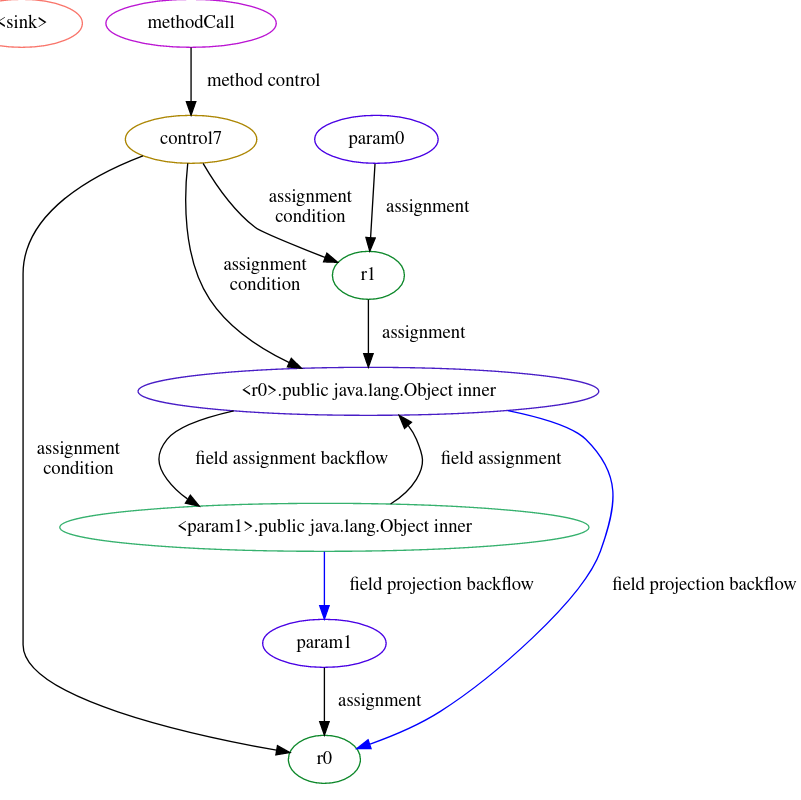
\includegraphics[scale=0.35]{screenshot20201231224543.png}
  \label{fig:param-to-param-lfg}
\end{figure}

Note the mutual flow between the nodes
\code{<r0>.public java.lang.Object.inner} and
\code{<param1>.public java.lang.Object.inner}.
Since \code{param1} is assigned into the local temporary \code{r0},
they point to the same value,
so their common field \code{inner} are located at the same address,
hence flow to one node always flows to the other.

\subsubsection{Control flow}
Branches and loops involve more \fnname{Control} nodes in the \ac{LFG}.

Consider the loop tests in Listing~\ref{lst:loop-tests}.
The \code{loopDec} method effectively copies \code{i} to \code{a},
leaking the parameter to return value by control flow.
The \fnname{Control} from branching by \code{i} covers the assignment of \code{a},
allowing it to reach the return path.
Similarly, the \code{whileCall} method uses
the return proxy node of \code{supplier.getAsBoolean()} to branch,
leaking any possible returned flow from \code{getAsBoolean()} to its own return path.

\IncludeCodePart{lst:loop-tests}
{../core/src/test/java/io/github/sof3/enclavlow/cases/lfg/LoopCase.java}
{Loop test cases}
{16}{30}

The test results can be reproduced with the Gradle test task.
Consult the GitHub CI setup at \url{https://github.com/SOF3/enclavlow/actions}
for details on environment setup.
Other unit tests in the project are omitted in this report
as their functionalities are insignificant or already covered by the above cases.

\subsection{Performance}
To analyze the performance of \pname{} in real projects,
a test application is written to run the \pname{} gradle plugin with.
The source code is available under the \code{example/} directory on the GitHub repository.
The test application opens a UDP socket that listens for packets
and computes a 6-digit one-time-password from the packet data.

The application involves the 6 simple methods of its own,
as well as the following methods from Java standard library:

\begin{itemize}
  \item \code{DatagramPacket.getData()}
  \item \code{DatagramPacket.new(byte[], int)}
  \item \code{DatagramPacket.setData(byte[])}
  \item \code{DatagramSocket.bind(InetSocketAddress)}
  \item \code{DatagramSocket.isClosed()}
  \item \code{DatagramSocket.new()}
  \item \code{DatagramSocket.receive(DatagramPacket)}
  \item \code{DatagramSocket.send(DatagramPacket)}
  \item \code{InetSocketAddress.new(String, int)}
  \item \code{System.currentTimeMillis()}
\end{itemize}

Due to transitive method calls,
it is found that 1806 different methods were eventually included in the analysis
(including native and abstract methods, which are not handled correctly;
see section \ref{subsec:difficulties-and-limitations} for details).
A total of 86 seconds were spent for analysis on an Intel i7-10510U CPU (1.80GHz)
(number of cores does not matter since the program is largely single-threaded)
on Linux kernel 5.4.0-58-generic with Java profiler enabled.

Profiler result shows that, among the 56 seconds of CPU time used on running Java code
(the remaining is attributed to JVM native operations),
76.8\% time is spent on \code{soot.SootResolver.resolveClass},
which is the part where Soot compiles the Java bytecode into its own representation.
Only 18.7\% time was actually spent on code from this project,
i.e. the part performing flow analysis.

Since Soot is not thread-safe due to its unfortunately aggressive use of static variables,
it is not possible to improve performance using parallelism.
Major change on the Soot framework or \ac{JVM} forking is necessary
for performance improvement.

Soot issues aside,
a large amount of CPU time is spent
on repacking the \ac{LFG} due to node removal.
A more efficient graph representation structure (such as layered views)
may be helpful in improving performance of this part.
Nonetheless, since this part only contributes a small proportion to the overall CPU time,
insignificant improvement is expected.

A full profiler report can be found at \code{docs/profiler-results.jfr} on the GitHub repository.
Figures \ref{fig:flame-graph-full} and \ref{fig:flame-graph-analysis}
show the flame graph of profiler samples.

\begin{figure}
  \caption{Profiler flame graph (full)}
  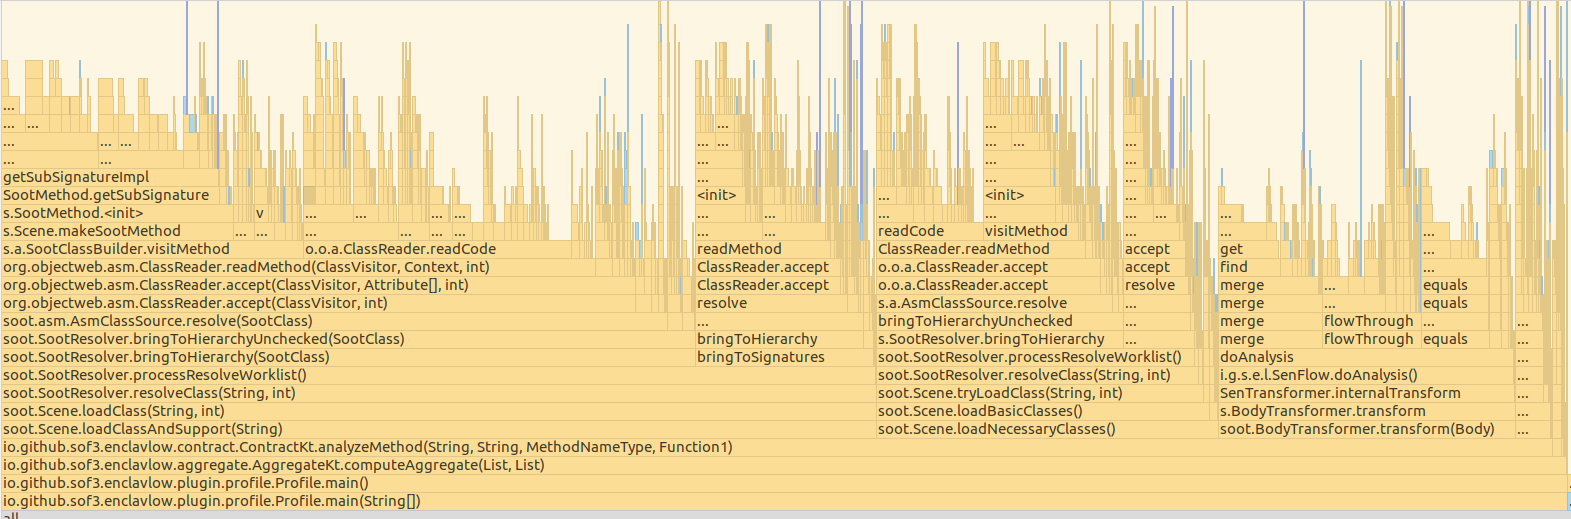
\includegraphics[scale=0.33]{screenshot20201231183130.png}
  \label{fig:flame-graph-full}
\end{figure}

\begin{figure}
  \caption{Profiler flame graph (analysis only)}
  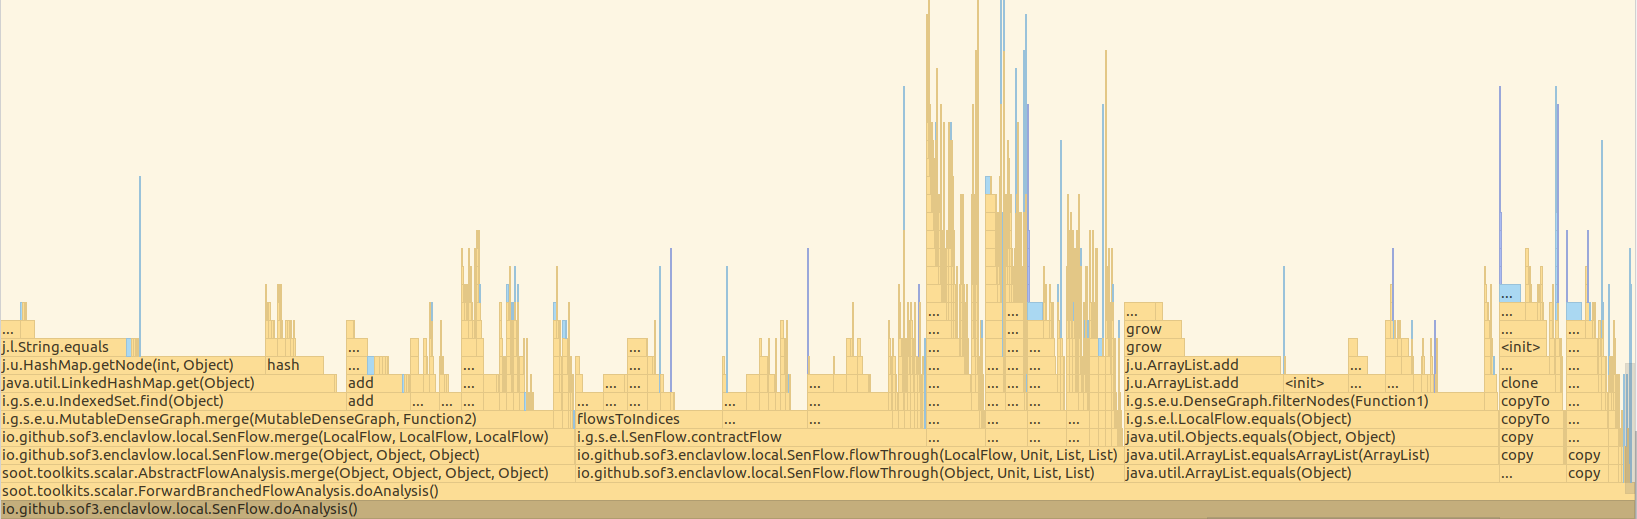
\includegraphics[scale=0.3]{screenshot20201231183716.png}
  \label{fig:flame-graph-analysis}
\end{figure}


\section{Discussion}\label{sec:discussion}
There are various unimplemented features in this project,
which can be tackled in future research.

\subsection{Limitations}\label{subsec:difficulties-and-limitations}
As is every code analysis system,
perfect detection is almost impossible.
This subsection will show that
the requirements of \pname{} is a \emph{superset} of the common analysis tools
in terms of problems to identify.

\subsubsection{Polymorphism}\label{subsubsec:polymorphism}
The principles of \ac{OOP} imply that the receiver of a method call
may be swapped with a compatible implementation in another subclass
that performs different actions than the current one.
Although Uranus prevents the adversary
from passing arbitrary malicious code into the enclave memory,
it is still possible to pass objects of unexpected but trusted subclass
through the \code{@JECall} boundary.
Alternatively, an alternative form of Iago attack
passes originally impossible combination of subtypes to the function,
which could also introduce attack vectors.
Consider Listing~\ref{lst:oop-subst-attack} for example.
If \code{cs} is passed with a \code{substr} implementation
that writes its parameters to a static variable,
the function would leak the length of the security-sensitive \code{secret},
which is not desirable.
To correctly solve the vulnerability of \ac{OOP} substitution,
it is necessary to perform call graph analysis on the actual classes passed to the method,
which involves more complex framework level work.

\IncludeCode{lst:oop-subst-attack}{./OopSubstAttack.java}
{Iago attack through substitution}{.6}{2.5}

Due to time constraints,
polymorphism handling is not implemented in this project.
Instead, a \emph{degenerate} contract graph
with the edge set $\left\{(\text{\fnname{Param}}~x, \text{\fnname{Return}}) : x\right\}$
is used as placeholder for abstract methods,
and possible subclass overrides are not yet considered.

\subsubsection{Native methods}\label{subsubsec:jni}
Similar to abstract methods,
\ac{JNI} methods are also not easy to analyze.
The implementation of \ac{JNI} methods is only available in the form of native dynamic libraries,
and reverse engineering such libraries is unnecessary, tedious and sometimes illegal.
A much simpler but accurate approach
is to analyze the native methods in the original languages they were written in,
integrating with tools such as Glamdring \cite{glamdring};
for the native methods within Java standard library,
it is possible to precompute the contract of each of them manually
and ship these with the software.
Similar to above, this task is omitted due to time constraints;
degenerate contracts are used as placeholder instead.
This assumption is inaccurate;
a common counterexample is the \code{System.arraycopy} method,
which leaks the values of the integer parameters into the destination array parameter
since the amount of elements changed leaks the integers involved.

\subsubsection{Duplicate code}\label{subsubsec:duplicate-code}
Despite optimizations and simplifications,
it is still not possible to perform perfectly accurate information flow analysis
within efficient time complexity~\cite{SmithGeoffrey2007PoSI}.
For example, this project merges conditional branches together
by taking the union of flow graphs,
resulting in easy false positive cases.
Listing~\ref{lst:known-false-positives} is an example of this:
the return statement appears in both arms,
so according to the mechanism explained above, the control flow shall leak
the branching condition \code{secret} to the return path.
Nevertheless, but the returned value is in fact always \code{x}.
Since this is a minor use case, this bug is considered not worth fixing.
In fact, duplicated code in multiple branch arms
is often regarded as an antipattern as well. % citation needed

\IncludeCode{lst:known-false-positives}{./KnownFalsePositives.java}
{False positive by duplicate code}{.6}{3}

Similarly, self-anonymized sensitive data are not identified correctly,
such as in Listing~\ref{lst:self-anonymized}.
It is believed that such errors are easy for a human to discover
and could be marked \code{sinkMarker} directly,
or simply copying \code{a} to another variable,
so these false positives do not have major effect on usability.
Note also that mutably sensitive data may be an antipattern
as the user may accidentally leak it in the future
by moving a line of code incorrectly.

\IncludeCode{lst:self-anonymized}{./SelfAnonymized.java}
{False positive by self-anonymization}{.6}{3}

\subsubsection{Implicit exceptions}
Apart from explicit \code{throw} statements,
runtime exceptions can also be raised when invalid operations are performed,
leaking information through control flow.
Consider Listing \ref{implicit-exceiption}.
While the mechanism of \pname{} does not discover any bugs,
the method throws an ArrayIndexOutOfBoundsException
if and only if \code{a >= index},
so an adversary could pass varying values for \code{a}
to binary-search the value of \code{index}.

\IncludeCode{implicit-exceiption}{./ImplicitException.java}
{Implicit exception}{.4}{3}

This is difficult to notice even for an alert developer.
Solutions are unfortunately usually achieved at the source code level,
such as using annotations like \code{@NotNull} and \code{@Size}.
As this project does not intend to reinvent the wheel,
prevention of such vulnerabilities is left as the task for other source-level tools.
In fact, such exceptions tend to cause other security issues in addition to enclave security,
well known as the "billion dollar problem" \cite{nullbillion}.
It is likely more efficient to try to avoid such unexpected behaviour
by fusing the source code before it gets compiled.

\subsubsection{Readability}
For the sake of consistency with Uranus,
it was originally intended to expose \code{sourceMarker} and \code{sinkMarker}
as annotations on local variables instead of method calls.
However, \ac{JLS} 9.6.1.2 explicitly stated that
\q{an annotation on a local variable declaration
is never retained in the binary representation}~\cite{jls},
so a method call based approach is used instead.
It is expected that \ac{JIT} optimization removes the cost
involved from an extra method call at \ac{JIT} compile time.

This also leads to readability issues.
The current HTML output is unable to reveal more information than the \ac{CFG}
because of the lack of information about the source code,
like local variable names and line numbers.
In the \ac{LFG}, generated variable names like \code{r0}
and control marker names like \code{control13} are used instead,
but they are not intuitive for the reader
and become hard to interpret when the method grows large.
The only solution for this problem is to provide additions at the source code level,
but since \pname{} takes inputs in the form of Java class binaries,
this is considered out of scope of the project.

\subsection{Recommended future research}\label{subsec:recommended-future-research}
There are multiple areas in which this project can be extended.

\pname{} applies handwritten heuristics to identify leaks.
Some special edges, such as field projection, are not very well-defined.
This reduces the reliability of \pname{} in terms of robustness in targeted attacks,
which is an important feature for security analysis.
A formal proof through tools like Coq~\cite{coq}
can be utilized to ensure that the \ac{LFG} construction does not miss marginal cases.

The project can also be used to improve Uranus performance.
Currently, to ensure enclave confidentiality,
Uranus requires enclave code accessing untrusted memory to
use Uranus's untrusted-memory \ac{API}
like \code{SafeGetField} and \code{SafeWriteField}\cite{uranus},
which checks the memory address against enclave bounds at runtime.
The static analysis in \pname{} allows Uranus to validate these bounds at compile time,
hence avoiding the runtime bounds-checking cost and improve performance.
Note that JIT optimization is not able to detect unnecessary bounds checking.
Since \code{enclavlow-core} exposes the \ac{AFG} result fully,
it shall be possible for the compiler in Uranus
to directly invoke this library to analyze the program being compiled.


\section{Conclusion}\label{sec:conclusion}
This project aims to develop a \ac{JVM} code analysis tool
for software using Uranus for \ac{SGX} applications
to assist the choice of enclave boundaries.
A divide-and-conquer approach was adopted for
efficient abstraction of information flow across a method.
Since the project delivers an analysis tool
but leaves the decision right to the user,
a higher tolerance for false positives was accepted.

To formalize the behaviour of false positives with the project,
analysis is to be conducted on the occurrence of false positives.
Usability of the tool with common libraries in the Java ecosystem will be assessed.
With sufficient theoretical background to support the correctness of the algorithms,
this tool is expected to serve as an auxiliary quality control integration
for open source projects that may see demand in the big data industry
and other confidential data processing applications.

The source code of this project is released at
\url{https://github.com/SOF3/enclavlow}.


\newpage
\addcontentsline{toc}{section}{References}
\begin{multicols}2
  \footnotesize
	\bibliographystyle{plain}
	\bibliography{cite}
\end{multicols}

\end{document}
